%=============================================================
%  EN2160 Electronic Design Realization
%  Final Report -- Restaurant Robot
%  (Autonomous Food Delivery Robot with Tabletop Request System)
%  Group: PENTAGON
%=============================================================
\documentclass[12pt,a4paper]{article}

%-------------------------------------------------------------
% Packages
%-------------------------------------------------------------
\usepackage[a4paper, top=25mm, bottom=25mm, left=25mm, right=25mm]{geometry}
\usepackage{graphicx}
\usepackage{amsmath}
\usepackage{amssymb}
\usepackage{booktabs}
\usepackage{array}
\usepackage{longtable}
\usepackage{listings}
\usepackage{xcolor}
\usepackage{caption}
\usepackage{subcaption}
\usepackage{hyperref}
\usepackage{fancyhdr}
\usepackage{titlesec}
\usepackage{setspace}
\usepackage{enumitem}
\usepackage{float}
\usepackage{multirow}
\usepackage{parskip}
\usepackage{siunitx}
\usepackage{tabularx}
\usepackage{arydshln}
\usepackage{colortbl}
\usepackage{tikz}
\usepackage{xcolor}
\usepackage{listings}
\lstset{
language=C,
basicstyle=\ttfamily\small,
keywordstyle=\color{blue!60!black},
commentstyle=\color{green!40!black},
numbers=left,
numberstyle=\tiny,
frame=single,
breaklines=true,
showstringspaces=false}
\usetikzlibrary{positioning,fit,arrows.meta}

%-------------------------------------------------------------
% Code listing style (place in the preamble, after xcolor/listings)
%-------------------------------------------------------------
\definecolor{codebg}{RGB}{245,245,245}
\definecolor{codekeyword}{RGB}{0,0,180}
\definecolor{codecomment}{RGB}{0,130,0}
\definecolor{codestring}{RGB}{163,21,21}
\definecolor{codenumber}{RGB}{128,128,128}

\lstdefinestyle{cstyle}{
  language=C,
  backgroundcolor=\color{codebg},
  basicstyle=\ttfamily\small,
  keywordstyle=\color{codekeyword}\bfseries,
  commentstyle=\color{codecomment}\itshape,
  stringstyle=\color{codestring},
  numberstyle=\tiny\color{codenumber},
  numbers=left,
  numbersep=8pt,
  frame=single,
  rulecolor=\color{gray!50},
  breaklines=true,
  showstringspaces=false,
  tabsize=2,
  captionpos=b
}

\lstset{style=cstyle}

%-------------------------------------------------------------
% Colours
%-------------------------------------------------------------
\definecolor{uomblue}{RGB}{0,51,102}

%-------------------------------------------------------------
% Header / footer
%-------------------------------------------------------------
\setlength{\headheight}{14pt}
\pagestyle{fancy}
\fancyhf{}
\renewcommand{\headrulewidth}{0.5pt}
\fancyhead[L]{\small\textcolor{uomblue}{Restaurant Robot}}
\fancyhead[R]{\small\textcolor{uomblue}{Final Report -- Group PENTAGON}}
\fancyfoot[C]{\thepage}

%-------------------------------------------------------------
% Section formatting -- \section acts as "Chapter"
%-------------------------------------------------------------
\titleformat{\section}{\Large\bfseries\color{uomblue}}{Chapter \thesection}{1em}{}[\titlerule]
\titleformat{\subsection}{\normalsize\bfseries\color{uomblue}}{\thesubsection}{1em}{}
\titleformat{\subsubsection}{\normalsize\itshape\color{uomblue}}{\thesubsubsection}{1em}{}

%-------------------------------------------------------------
% Hyperref
%-------------------------------------------------------------
\hypersetup{
  colorlinks=true,
  linkcolor=uomblue,
  urlcolor=uomblue,
  citecolor=uomblue,
  pdftitle={Restaurant Robot -- Final Report -- Group PENTAGON},
  pdfauthor={Group PENTAGON}
}

% Convenience command for placeholder figures - once you have the
% real image, delete the placeholderfig call and use a normal figure
% environment with \includegraphics instead.
\newcommand{\placeholderfig}[2]{%
  \begin{figure}[H]
    \centering
    \fbox{\parbox[c][5cm][c]{0.65\textwidth}{\centering\itshape #1}}
    \caption{#2}
  \end{figure}
}

% Convenience command for a real figure sourced from the team's own
% slides/renders, stored in the figs/ subfolder next to this .tex file.
\newcommand{\slidefig}[3][0.65\textwidth]{%
  \begin{figure}[H]
    \centering
    \includegraphics[width=#1]{#2}
    \caption{#3}
  \end{figure}
}

%=============================================================
\begin{document}
%=============================================================

%-------------------------------------------------------------
% COVER PAGE
%-------------------------------------------------------------
\thispagestyle{empty}
\begin{center}
  \vspace*{3mm}
  \rule{\linewidth}{1pt}\\[4mm]
  {\large\bfseries University of Moratuwa}\\[2mm]
  {\normalsize Faculty of Engineering}\\[1mm]
  {\normalsize Department of Electronic \& Telecommunication Engineering}\\[1mm]
  {\normalsize EN2160 -- Electronic Design Realization}\\[1mm]
  \rule{\linewidth}{0.5pt}\\[1mm]

  
\includegraphics[width=0.35\textwidth]{UOM Logo.png}\\[6mm]

  {\LARGE\bfseries\color{uomblue} Restaurant Robot}\\[4pt]
  {\large Autonomous Food Delivery Robot with Tabletop Request System}\\[4pt]
  {\normalsize\itshape Reducing Staff Workload \& Improving Service Speed}\\[10mm]

  {\Large\bfseries Final Project Report}\\[12mm]

  {\large\bfseries Group: PENTAGON}\\[6mm]

  \begin{tabular}{ll}
    \toprule
    \textbf{Index No.} & \textbf{Name} \\
    \midrule
    230016      & Abishek L.        \\
    230334V     & Hakam M.R.A       \\
    230449N     & Nuwanaka W.A.S    \\
    230581K     & Santhosh S        \\
    230654M     & Umair A           \\
    \bottomrule
  \end{tabular}\\[14mm]

  {\normalsize Submitted on: \today}
\end{center}
\newpage

%-------------------------------------------------------------
% ABSTRACT
%-------------------------------------------------------------
\thispagestyle{empty}
\section*{Abstract}
\addcontentsline{toc}{section}{Abstract}

The hospitality industry continues to face increasing operational costs, staff shortages, and growing customer expectations for faster and more efficient service. To address these challenges, this project presents the design, implementation, and evaluation of the \textbf{Restaurant Robot}, an integrated restaurant automation system developed for the EN2160 Electronic Design Realization module. The system comprises two interconnected subsystems: an autonomous food delivery robot that transports meals from the kitchen to designated tables by following a magnetic guide path, and a tabletop customer request device that enables diners to request water, tissues, the bill, or staff assistance through a simple button interface. The complete system integrates embedded hardware, wireless communication, custom printed circuit boards, firmware, mechanical enclosure design using SolidWorks, and a mobile application to provide a reliable and low-cost automation solution suitable for restaurant environments. The integrated system incorporates magnetic line-following, obstacle detection, weight sensing, automatic charging, Wi-Fi-based communication, and real-time request handling to ensure safe and efficient operation while reducing the workload of restaurant staff. This report presents the complete engineering process, including problem identification, requirement analysis, system architecture, component selection, circuit and PCB design, firmware development, mechanical design, prototype realization, testing, cost analysis, and commercialization considerations. The completed prototype successfully demonstrates the integration of embedded systems, electronics, wireless communication, firmware, and mechanical design into a practical, scalable, and cost-effective solution for modern restaurant automation.

\newpage

%-------------------------------------------------------------
% TABLE OF CONTENTS / FIGURES / TABLES
%-------------------------------------------------------------
\tableofcontents
\newpage
%=============================================================
\section{Introduction}
%=============================================================

\slidefig{Existing Workflow}{Existing manual food delivery workflow in a typical restaurant.}

\subsection{Background}

Recent advancements in embedded systems, wireless communication, sensor technology, and autonomous mobile robotics have significantly accelerated the adoption of automation across various service industries. Among these, the hospitality sector has increasingly embraced service robots to improve operational efficiency, reduce staff workload, and enhance the overall customer experience. Autonomous food delivery robots are now widely deployed in restaurants, hotels, and food courts across countries such as Japan, China, South Korea, and Singapore, where they assist staff by transporting meals, guiding customers, and performing other repetitive service tasks.

Modern restaurant robots typically integrate embedded controllers, wireless communication, intelligent sensing, motor control, and autonomous navigation to perform safe and reliable operation in dynamic indoor environments. Depending on the application, navigation methods range from magnetic guide paths and QR-code localization to LiDAR- and vision-based simultaneous localization and mapping (SLAM). While high-end commercial solutions offer advanced capabilities, they are often expensive and require significant infrastructure and maintenance costs, making them less accessible for small and medium-sized businesses.

In Sri Lanka, the adoption of restaurant automation remains limited, primarily due to the high cost of imported robotic systems and the lack of affordable locally developed alternatives. However, the increasing availability of low-cost embedded platforms, custom PCB fabrication, wireless communication technologies, and rapid prototyping tools such as SolidWorks and 3D printing has created new opportunities for developing practical and cost-effective automation solutions. This project was therefore undertaken to design and implement a locally developed restaurant service robot capable of reducing staff workload, improving service efficiency, and demonstrating the practical application of embedded system engineering in a real-world hospitality environment.

\subsection{Motivation}

The hospitality industry is experiencing increasing pressure due to rising labour costs, workforce shortages, and growing customer expectations for faster, more reliable, and consistent service. During peak operating hours, restaurant staff must simultaneously manage food delivery, customer requests, billing, and table maintenance, often resulting in longer waiting times, increased workload, and reduced customer satisfaction. Automating repetitive tasks such as food transportation and customer service requests can significantly improve operational efficiency while allowing staff to focus on customer interaction and higher-value responsibilities.

To better understand these challenges, a pre-project survey involving 79 respondents was conducted. The survey revealed that only 6\% of respondents rated current restaurant service speed as excellent, while 66\% rated it 3 out of 5 or lower. Furthermore, 71.4\% of respondents described restaurant service speed as only ``moderate,'' indicating considerable room for improvement. The survey also highlighted delays in responding to customer requests during busy periods, reinforcing the need for a more efficient service management system.

Motivated by these findings, this project aims to develop a low-cost, modular restaurant automation system capable of improving service speed, reducing staff workload, and enhancing the overall dining experience. Rather than replacing human workers, the proposed system is intended to assist restaurant staff by automating routine delivery and communication tasks, thereby enabling more efficient and customer-focused restaurant operations.

\subsection{Problem Statement}

Restaurant operations face several operational challenges that reduce
service efficiency, increase staff workload, and negatively impact the
overall customer experience. To better understand these issues, the
team conducted a comparative analysis of conventional restaurant
operations together with a customer survey involving 79 respondents.
The key problems identified are summarized below.

\begin{itemize}[nosep]
    \item Restaurant staff spend an estimated 30--40\% of their working
    time transporting food from the kitchen to customer tables,
    reducing the time available for customer interaction and other
    service-related tasks.

    \item The average food delivery time in a conventional restaurant
    is approximately 5--8 minutes, whereas the proposed autonomous
    delivery system is designed to reduce this to approximately
    2--3 minutes.

    \item Restaurant staff may walk more than 15,000 steps per day
    while delivering food and responding to customer requests. The
    proposed system aims to reduce this workload to fewer than
    5,000 steps per day by automating routine delivery tasks.

    \item Manual food delivery is susceptible to order delivery errors,
    with an estimated error rate of 5--8\%. The proposed system is
    designed to reduce this error rate to below 1\% through guided
    autonomous navigation and controlled delivery.

    \item Customer waiting time increases significantly during peak
    operating hours. According to the survey, 71.4\% of respondents
    reported experiencing delays in food delivery during busy periods.

    \item Approximately 71.4\% of respondents indicated that restaurant
    staff sometimes fail to notice customer requests, such as requests
    for water, tissues, the bill, or staff assistance. This highlights
    the need for a dedicated tabletop request system that enables
    reliable communication between customers and restaurant staff.
\end{itemize}

The findings from the comparative study and customer survey clearly
indicate that improving restaurant service requires more than simply
reducing food delivery time. An effective solution must also reduce
staff workload, improve responsiveness to customer requests, minimize
delivery errors, and enhance overall operational efficiency. These
identified challenges directly motivated the design and development of
the proposed Restaurant Robot and its integrated tabletop customer
request system.

\begin{figure}[H]

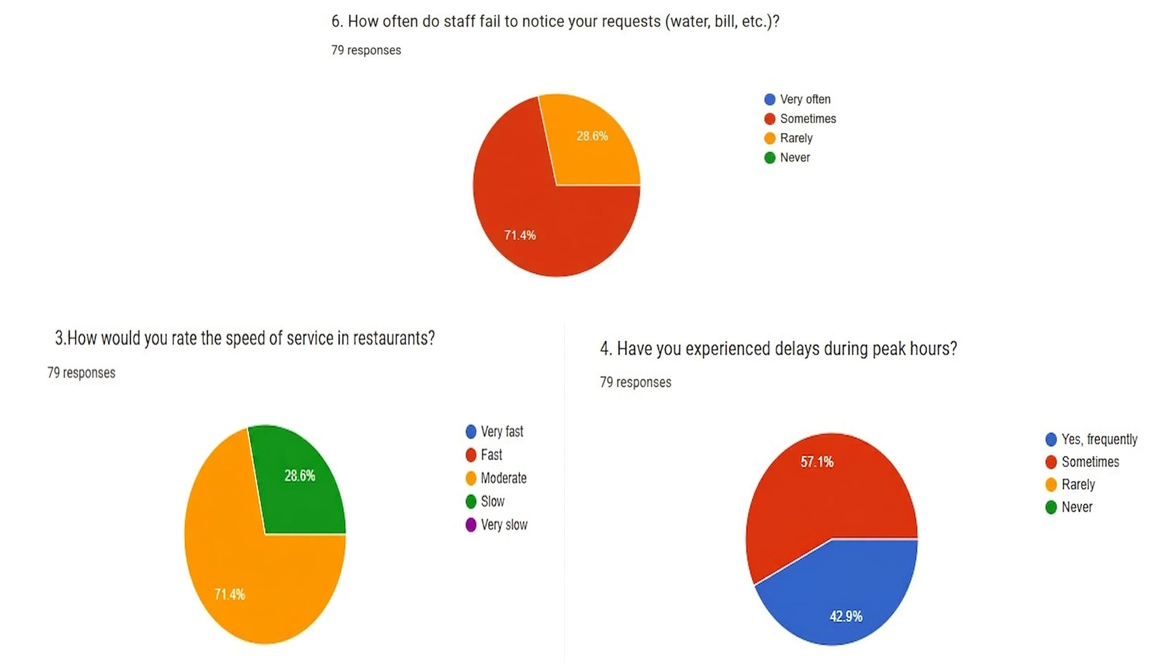
\includegraphics[width=1\textwidth]{fig1.png}
\caption{Customer survey results on perceived restaurant service speed and delays during peak hours.}
\label{fig:comparison}
\end{figure}

\subsection{Stakeholder Analysis}

The proposed Restaurant Robot system involves several stakeholders,
each with different expectations and requirements. Understanding these
stakeholders was essential for defining the system requirements and
ensuring that the final design provides practical value to all users.

\begin{itemize}[nosep]
    \item \textbf{Customers:} Customers are the primary beneficiaries
    of the system. They expect fast, reliable, and convenient service
    with minimal waiting time. The autonomous delivery robot and
    tabletop request device enable quicker food delivery, simplified
    service requests, and an improved overall dining experience.

    \item \textbf{Restaurant Owners:} Restaurant owners seek solutions
    that improve operational efficiency while minimizing long-term
    labour costs. The proposed system assists in reducing staff
    workload, improving service consistency, increasing customer
    satisfaction, and providing an innovative feature that can
    differentiate the restaurant from competitors.

    \item \textbf{Waitstaff:} Waitstaff are responsible for serving
    customers and responding to their requests throughout restaurant
    operations. By automating repetitive food delivery tasks and
    digitally displaying customer requests, the system reduces
    unnecessary walking, improves task prioritization, and allows staff
    to focus on customer interaction and service quality.

    \item \textbf{Kitchen Staff:} Kitchen staff require an efficient
    method for dispatching completed orders without depending on the
    immediate availability of waitstaff. The proposed system allows
    food to be loaded onto the robot and dispatched directly to the
    assigned table, reducing delays between food preparation and
    delivery.

    \item \textbf{System Developers and Maintenance Personnel:}
    Engineers and maintenance personnel require a system that is
    modular, reliable, and easy to troubleshoot. The use of a custom
    PCB, modular firmware, standardized electronic components, and a
    well-organized mechanical design simplifies maintenance, future
    upgrades, and component replacement.
\end{itemize}

The requirements of these stakeholders directly influenced the system
architecture, hardware selection, firmware development, and mechanical
design decisions adopted throughout the project.

\subsection{Objectives}

The primary objective of this project is to design and implement an
autonomous restaurant service robot capable of improving operational
efficiency, reducing staff workload, and enhancing the overall dining
experience. To achieve this objective, the system was designed to
satisfy the following functional and non-functional requirements.

\subsubsection*{Functional Objectives}

\begin{itemize}[nosep]
    \item Develop an autonomous mobile robot capable of transporting
    food from the kitchen to a designated customer table by following
    a magnetic guide path while safely detecting and avoiding
    obstacles.

    \item Detect the loading and unloading of food trays using an
    onboard weight sensing mechanism to ensure reliable delivery
    operation.

    \item Provide customers with a tabletop request device that allows
    them to request water, tissues, the bill, or staff assistance
    through a simple button interface.

    \item Enable kitchen staff to assign delivery destinations through
    a mobile application, allowing the robot to autonomously navigate
    to the selected table.

    \item Automatically return to the charging station after completing
    deliveries or when the battery level falls below a predefined
    threshold.

    \item Establish reliable wireless communication between the robot,
    tabletop request device, and mobile application for real-time
    coordination and status updates.
\end{itemize}

\subsubsection*{Non-Functional Objectives}

\begin{itemize}[nosep]
    \item Develop a cost-effective prototype using commercially
    available electronic components while maintaining a significantly
    lower cost than imported commercial restaurant service robots.

    \item Ensure stable, reliable, and low-latency Wi-Fi communication
    between all system components during normal operation.

    \item Achieve smooth and stable robot motion to minimize vibration
    and prevent food spillage during transportation.

    \item Design a robust mechanical structure capable of withstanding
    continuous operation in a restaurant environment while remaining
    easy to clean and maintain.

    \item Develop a modular hardware and firmware architecture that
    simplifies troubleshooting, maintenance, and future system
    expansion.

    \item Prioritize safe system operation through reliable obstacle
    detection, controlled motor operation, and automatic charging
    functionality.
\end{itemize}

\subsection{Scope}

The scope of this project is limited to the design, implementation,
and evaluation of an autonomous restaurant service robot intended for
indoor restaurant environments with a predefined magnetic guide path.
The developed system comprises an autonomous food delivery robot, a
tabletop customer request device, a staff-facing mobile application,
and a charging station that together provide an integrated restaurant
automation solution.

The robot is designed to transport food from the kitchen to designated
customer tables by following a magnetic guide path while detecting
obstacles and automatically returning to its charging station when
idle or when the battery level is low. The tabletop request device
enables customers to request water, tissues, the bill, or staff
assistance, while the mobile application allows restaurant staff to
assign delivery destinations and monitor the operational status of the
robot.

The project does not include autonomous mapping or navigation in
unstructured environments, computer vision-based localization,
multi-robot coordination, online payment processing, inventory
management, or integration with third-party Point-of-Sale (POS)
systems. These advanced capabilities require additional hardware,
software, and infrastructure that are beyond the scope of the EN2160
Electronic Design Realization project and are therefore identified as
potential future enhancements in
Chapter~\ref{sec:future}.

%=============================================================
\section{System Architecture}
%=============================================================

\subsection{Overall Architecture}

The Restaurant Robot system adopts a centralized embedded architecture
based on the ESP32-S3 microcontroller, which serves as the primary
control unit for all sensing, processing, communication, and actuator
operations. The complete system consists of four interconnected
subsystems: the autonomous food delivery robot, the tabletop customer
request device, the staff-facing mobile application, and the charging
station. Together, these subsystems provide an integrated solution for
restaurant service automation.

\slidefig[0.95\textwidth]{123}{Overall system architecture illustrating the ESP32-S3 control unit, sensing modules, actuator interfaces, power subsystem, wireless communication, tabletop request device, and staff mobile application.}

As illustrated in Figure 3, the ESP32-S3 acts as
the central controller by continuously acquiring data from the Hall
effect sensors, ultrasonic sensors, and load cell module to determine
the robot's position, detect obstacles, and verify food loading or
unloading. Based on this information, the controller executes the
navigation and delivery algorithms while generating appropriate control
signals for the motor driver, display, status LEDs, and audible
indicators.

Wireless communication is established through the ESP32-S3's integrated
Wi-Fi interface, enabling real-time data exchange between the robot,
the tabletop customer request device, and the staff mobile
application. This communication allows customer requests to be
forwarded to restaurant staff, delivery destinations to be assigned,
and operational status information to be monitored throughout the
delivery process.

A dedicated power subsystem supplies regulated voltages to the
electronic components while the rechargeable battery provides portable
operation. Upon completing a delivery or when the battery level falls
below a predefined threshold, the robot automatically returns to the
charging station for battery recharging. The detailed hardware
implementation of each subsystem is presented in the following
chapters.

\subsection{System Operation}
The end-to-end operational flow is as follows:
\begin{enumerate}[nosep]
  \item Customer presses a request button on the tabletop device
  (water, tissue, bill, or staff assistance).
  \item The request is transmitted over Wi-Fi and received by staff
  through the mobile app.
  \item Once an order is ready, kitchen staff assign the table to the
  robot via the app.
  \item The robot navigates to the assigned table by following the
  magnetic guide tape using its Hall effect sensor array.
  \item The onboard ultrasonic sensors continuously check for
  obstacles; the robot stops and waits if the path is blocked, then
  resumes.
  \item The weight sensor confirms the tray has been loaded before
  departure and unloaded on arrival.
  \item The robot returns to the magnetic charging station and docks
  automatically when idle.
\end{enumerate}

\subsection{Alternative Designs}

Three navigation approaches were considered for the delivery robot.

\begin{table}[H]
\centering
\caption{Comparison of navigation alternatives considered.}
\renewcommand{\arraystretch}{1.3}
\begin{tabular}{@{}p{3cm}p{5.5cm}p{5.5cm}@{}}
\toprule
\textbf{Approach} & \textbf{Advantages} & \textbf{Disadvantages} \\
\midrule
Manual Service (Baseline) & No hardware or development cost; maximum flexibility & Does not address labour shortages or service consistency \\

Full AGV/SLAM Navigation & Flexible routing; no fixed guide-path infrastructure required & High development cost and complexity; requires more powerful computing and sensing (LiDAR/cameras); longer development time \\

Magnetic Tape Line Following & Simple, low-cost, and reliable within a fixed restaurant layout; unaffected by floor colour or ambient lighting (unlike IR-based line following); rapid development within the module timeline & Requires a fixed guide path; less flexible if the restaurant layout changes \\
\bottomrule
\end{tabular}
\end{table}

Magnetic tape line following using Hall effect sensors was selected
over IR-based line following because it is unaffected by floor colour
or ambient lighting conditions, providing more reliable path tracking
in a restaurant environment while remaining significantly simpler and
more cost-effective than full autonomous navigation.

%=============================================================
\section{Requirement Analysis}
%=============================================================

\subsection{Functional Requirements}

Table~\ref{tab:functional_requirements} summarizes the functional
requirements of the proposed Restaurant Robot system.

\begin{table}[H]
\centering
\caption{Functional requirements.}
\label{tab:functional_requirements}
\renewcommand{\arraystretch}{1.2}
\begin{tabular}{@{}p{1.2cm}p{11.3cm}@{}}
\toprule
\textbf{ID} & \textbf{Requirement} \\
\midrule
FR1 & The robot shall autonomously follow a magnetic guide path from the kitchen to the assigned customer table. \\

FR2 & The robot shall detect obstacles along its path and stop safely until the path is clear. \\

FR3 & The robot shall detect tray loading and unloading using an onboard weight sensor. \\

FR4 & The tabletop request device shall enable customers to request water, tissues, the bill, or staff assistance. \\

FR5 & Kitchen staff shall be able to assign a delivery destination to the robot through the mobile application. \\

FR6 & The robot shall automatically return to the charging station and recharge when idle or when the battery level falls below a predefined threshold. \\
\bottomrule
\end{tabular}
\end{table}

\subsection{Non-Functional Requirements}

Table~\ref{tab:nonfunctional_requirements} summarizes the non-functional
requirements of the proposed Restaurant Robot system.

\begin{table}[H]
\centering
\caption{Non-functional requirements.}
\label{tab:nonfunctional_requirements}
\renewcommand{\arraystretch}{1.2}
\begin{tabular}{@{}p{2.8cm}p{9.7cm}@{}}
\toprule
\textbf{Category} & \textbf{Requirement} \\
\midrule
Accuracy &
The robot shall reliably follow the magnetic guide path regardless of floor colour or ambient lighting conditions. \\

Battery Life &
The robot shall operate continuously for approximately 8--10 hours on a single charge and support a recharge time of approximately 4--5 hours. \\

Speed &
The robot shall maintain a travel speed of approximately 0.3--0.5~m/s, providing efficient delivery while ensuring stable food transportation. \\

Reliability &
The Wi-Fi communication between the robot, tabletop request device, and mobile application shall remain stable and reliable under normal restaurant operating conditions. \\

Safety &
The robot shall stop immediately when an obstacle is detected and resume operation only after the path is clear. \\

Maintainability &
The system shall employ a modular hardware and firmware architecture to simplify maintenance, troubleshooting, and future upgrades. \\
\bottomrule
\end{tabular}
\end{table}

\subsection{System Specifications}

Figure 4 and
Table~\ref{tab:system_specifications} summarize the key specifications
of the proposed Restaurant Robot system.

\slidefig{product_specification}{Summary of the proposed Restaurant Robot specifications.}

\begin{table}[H]
\centering
\caption{System hardware specifications.}
\label{tab:system_specifications}
\renewcommand{\arraystretch}{1.2}
\begin{tabular}{@{}p{5cm}p{7.5cm}@{}}
\toprule
\textbf{Parameter} & \textbf{Specification} \\
\midrule
Overall dimensions & 50~cm $\times$ 40~cm $\times$ 120~cm \\

Maximum payload & 12--15~kg \\

Navigation method & Magnetic guide path using Hall effect sensors \\

Obstacle detection & Ultrasonic sensors (HC-SR04) \\

Travel speed & 0.3--0.5~m/s \\

Battery operating time & 8--10 hours \\

Battery charging time & 4--5 hours \\

Construction materials & ABS plastic (base/chassis) and wood (upper shelving) \\

Main controller & ESP32-S3-WROOM-1-N16R2 \\

Communication & Wi-Fi (Robot $\leftrightarrow$ Mobile Application $\leftrightarrow$ Tabletop Request Device) \\
\bottomrule
\end{tabular}
\end{table}

%=============================================================
\section{Hardware Design}
%=============================================================

The hardware architecture was designed by evaluating multiple
components for each subsystem based on performance, reliability,
cost, power consumption, and ease of integration. The selected
components provide a balance between functionality and affordability
while satisfying the system requirements.

%-------------------------------------------------------------
\subsection{Main Controller}
%-------------------------------------------------------------

\slidefig{microcontroller}{Microcontrollers used in the Restaurant Robot hardware design.}

The Restaurant Robot utilizes two microcontrollers:
the \textbf{ESP32-S3-WROOM-1-N16R2} and the
\textbf{STM32F103C8T6}. The ESP32-S3 provides built-in Wi-Fi and
Bluetooth connectivity, a dual-core processor, and sufficient GPIO pins
for communication and high-level control.

The STM32F103C8T6 is used for real-time hardware control due to its
multiple GPIO pins, low power consumption, and reliable peripheral
interfaces. This dual-controller architecture improves system
performance, reliability, and modularity.

%-------------------------------------------------------------
\subsection{Sensors}
%-------------------------------------------------------------

\slidefig{sensor}{Selected sensing components for navigation, weight measurement, and obstacle detection.}

\textbf{Line Following -- Hall Effect Sensor (SS49E):}
The SS49E Hall effect sensor was selected instead of IR-based line
following because it detects the magnetic guide path reliably,
regardless of floor colour or ambient lighting conditions, while
providing a simple analogue output for accurate path tracking.

\vspace{0.5em}

\textbf{Weight Sensing -- Load Cell with HX711 Amplifier:}
A load cell with an HX711 amplifier was selected instead of an
IR-based detection method because it directly measures the weight of
the food tray, allowing reliable detection of both loading and
unloading events regardless of the tray material or colour.

\vspace{0.5em}

\textbf{Obstacle Detection -- HC-SR04 Ultrasonic Sensor:}
The HC-SR04 ultrasonic sensor was selected instead of LiDAR- or
camera-based solutions because it offers a low-cost, reliable, and
computationally efficient method of obstacle detection while operating
independently of ambient lighting conditions.

%-------------------------------------------------------------
\subsection{Body and Motion}
%-------------------------------------------------------------

\slidefig{fig 123}{Selected motors, motor driver, and enclosure materials.}

\textbf{Motors -- JGB37-520 DC Gear Motor:}
The JGB37-520 DC gear motor was selected over the JA27-320 and
JGB320-555 alternatives due to its high torque output, self-locking
characteristics that prevent roll-back when stationary, and integrated
encoder, which provides the possibility of future closed-loop position
control.

\vspace{0.5em}

\textbf{Motor Driver -- L298N Dual H-Bridge:}
The L298N motor driver was selected instead of the TB6612FNG because
it supports the 12V motor supply, delivers up to 2A continuous current
per channel, is inexpensive and widely available, and can be directly
controlled using PWM signals generated by the ESP32-S3.

\vspace{0.5em}

\textbf{Enclosure Materials:}
The chassis base is constructed from ABS plastic, while the upper
shelving is fabricated from wood. This combination was selected over
an entirely ABS construction to provide a balance between structural
strength, reduced material cost, ease of fabrication, and overall
mechanical stability.

%-------------------------------------------------------------
\subsection{Power System}
%-------------------------------------------------------------

\slidefig{1111}{Battery, voltage regulation, and charging system.}

The robot is powered by a \textbf{12V 9000mAh Li-ion battery pack},
chosen for its high energy density, lightweight design, and long
operating life.

An \textbf{LM2596} buck converter provides the 5V supply for the
ESP32-S3 and other peripherals, while an \textbf{AMS1117} regulator
generates the 3.3V supply for low-voltage devices.

Battery charging is implemented using a \textbf{magnetic pogo-pin
charging station}, providing reliable electrical contact, automatic
alignment, and a simple charging solution.

%-------------------------------------------------------------
\subsection{User Output}
%-------------------------------------------------------------

\slidefig{component_user_output}{Selected user output components.}

\textbf{Buzzer -- 5V Passive Buzzer:}
A 5V passive buzzer was selected instead of an active buzzer because
it supports programmable tone generation, enabling multiple audible
alert patterns for different system states while maintaining low power
consumption and a compact form factor.

\vspace{0.5em}

\textbf{Display -- I\textsuperscript{2}C OLED (128$\times$64):}
The I\textsuperscript{2}C OLED display was selected instead of an SPI
TFT LCD because it requires only two communication lines, consumes
less power, provides sufficient resolution for system status
information, and remains clearly visible under typical restaurant
lighting conditions.

\vspace{0.5em}

\textbf{LED Indicators -- WS2812B Addressable LED Strip with 74HC595
Shift Register:}
The WS2812B addressable LED strip was selected instead of conventional
single-colour LEDs because it provides programmable multi-colour
status indication using a single control signal. The 74HC595 shift
register expands the available output pins, reducing the GPIO
requirements of the ESP32-S3 while simplifying control of additional
status indicators.

%=============================================================
\section{Electronic Circuit Design}
%=============================================================

The complete circuit was designed in Altium Designer and implemented
as a custom two-board PCB consisting of a main controller board and a
74HC595 expansion board.

\slidefig[0.95\textwidth]{xyz}{Complete circuit schematic captured in Altium Designer: main controller board (left) and 74HC595 expansion board (right).}

\subsection{Power Circuit}

The 12V battery supply is regulated by an LM2596 switching regulator
to generate the 5V rail and an AMS1117 regulator to generate the 3.3V
rail. Decoupling capacitors are placed at the output of each regulator
to improve supply stability.

\subsection{Motor Driver Circuit}

The L298N dual H-bridge motor driver is interfaced with the ESP32-S3
through PWM and direction control signals and drives the two
JGB37-520 DC gear motors via screw-terminal connectors.

\subsection{Sensor Circuit}

The Hall effect sensor array, HC-SR04 ultrasonic sensors, and
HX711-based load cell interface are connected to dedicated headers on
the main controller board. Since the HC-SR04 echo signal operates at
5V while the ESP32-S3 GPIO operates at 3.3V, a voltage divider is used
to reduce the echo signal to a safe logic level.

\subsection{LED / Shift-Register Circuit}

Six cascaded 74HC595 shift registers expand the available digital
outputs, allowing multiple LED indicators to be controlled using a
small number of ESP32-S3 GPIO pins.

\subsection{Wireless Communication}

Wireless communication is provided by the ESP32-S3's integrated Wi-Fi
module; therefore, no external Wi-Fi module is required.

\section{Firmware}
\label{subsec:firmware}

The robot firmware coordinates motor control, magnetic-line navigation, route
execution, turning, fault recovery, docking, and communication with the web
application. Sensor feedback is obtained from a seven-channel Hall-effect
array, two wheel encoders, an MPU6050 inertial measurement unit (IMU), and a
digital charger-detection input. The code examples in this section are
simplified extracts of the implemented control logic and are included to show
the main operating principles.

\subsubsection{State-Machine Architecture}

The navigation software is organised as a non-blocking state machine. This
allows the controller to update sensors, receive commands, apply motor outputs,
and perform safety checks continuously. Each state represents one bounded
operation, such as following a line, positioning the axle, turning, recovering
the line, waiting at a table, or docking.

\begin{lstlisting}[caption={Simplified navigation state machine.},label={lst:nav-state}]
typedef enum {
    NAV_IDLE,
    NAV_FOLLOW_LINE,
    NAV_POSITION_AXLE,
    NAV_TURNING,
    NAV_FIND_LINE,
    NAV_AT_TABLE,
    NAV_RETURNING,
    NAV_DOCKING,
    NAV_OBSTACLE_STOP,
    NAV_ERROR
} NavigationState;

void updateNavigation(void)
{
    updateHallSensors();
    updateEncoders();
    updateMpuYaw();
    checkSafetyInputs();

    switch (navigationState) {
        case NAV_FOLLOW_LINE:   followCurrentSegment(); break;
        case NAV_POSITION_AXLE: positionAxleOnNode();   break;
        case NAV_TURNING:       updateTurn();            break;
        case NAV_FIND_LINE:     recoverMagneticLine();   break;
        case NAV_DOCKING:       updateDocking();         break;
        default:                stopMotors();             break;
    }
}
\end{lstlisting}

\subsubsection{Magnetic-Line Detection and PID Steering}

The seven analogue Hall sensors are calibrated while the robot is away from
the magnetic line. During operation, the firmware calculates the absolute
difference between each reading and its stored baseline. A weighted average of
the active sensors estimates whether the line is to the left or right of the
robot. The resulting error is passed to a PID controller, which adjusts the two
motor PWM values in opposite directions.

\begin{lstlisting}[caption={Hall-array processing and differential PID control.},label={lst:hall-pid}]
float calculateLineError(void)
{
    const int8_t positionWeight[7] = {-3, -2, -1, 0, 1, 2, 3};
    float weightedStrength = 0.0f;
    float totalStrength = 0.0f;

    for (uint8_t i = 0; i < 7; i++) {
        hallStrength[i] = abs(hallRaw[i] - hallBaseline[i]);

        if (hallStrength[i] >= HALL_THRESHOLD) {
            weightedStrength += positionWeight[i] * hallStrength[i];
            totalStrength += hallStrength[i];
        }
    }

    if (totalStrength == 0.0f)
        return lastLineError;

    lastLineError = weightedStrength / totalStrength;
    return lastLineError;
}

void followLinePid(void)
{
    float error = calculateLineError();
    float derivative = error - previousError;
    integralError += error;

    float correction = (KP * error) +
                       (KI * integralError) +
                       (KD * derivative);

    int leftPwm  = BASE_PWM + correction;
    int rightPwm = BASE_PWM - correction + RIGHT_MOTOR_TRIM;

    setMotorPwm(constrain(leftPwm,  0, MAX_PWM),
                constrain(rightPwm, 0, MAX_PWM));
    previousError = error;
}
\end{lstlisting}

A short line-loss confirmation time prevents the controller from reacting to
small field gaps between adjacent magnetic poles. Perpendicular magnetic
markers are accepted only when their sensor pattern remains valid for a minimum
confirmation period and the robot is inside the expected encoder-distance
window.

\subsubsection{Encoder Distance and Node Verification}

The left and right quadrature encoders measure the progress of each route
segment. The average wheel count is converted to centimetres using an
experimentally calibrated count-per-centimetre value. Encoder distance is used
as a verification window rather than the robot's only position source, because
wheel slip and turns can introduce cumulative error.

\begin{lstlisting}[caption={Encoder distance and expected-node window.},label={lst:encoder-window}]
float getTravelledDistanceCm(void)
{
    int32_t left  = abs(leftEncoderCount  - segmentLeftStart);
    int32_t right = abs(rightEncoderCount - segmentRightStart);
    float averageTicks = 0.5f * (left + right);

    return averageTicks / ENCODER_TICKS_PER_CM;
}

bool nodeIsInsideWindow(float expectedDistanceCm)
{
    float distance = getTravelledDistanceCm();

    return distance >= expectedDistanceCm - NODE_WINDOW_BEFORE_CM &&
           distance <= expectedDistanceCm + NODE_WINDOW_AFTER_CM;
}

if (nodePatternConfirmed() && nodeIsInsideWindow(segmentLengthCm)) {
    stopMotors();
    navigationState = NAV_POSITION_AXLE;
}
\end{lstlisting}

After the front Hall array detects a turning marker, the robot advances by the
calibrated sensor-to-axle distance. This places the drive-wheel axis near the
physical node before the turn begins. The encoder count is reset when the next
route segment starts.

\subsubsection{IMU-Assisted Turning and Heading Verification}

The MPU6050 gyroscope is calibrated while the robot is stationary at the dock.
Yaw is integrated continuously during the mission. At the beginning of each
turn, the firmware records the current yaw and measures the turn relative to
this value. Therefore, a 90-degree or 180-degree turn does not depend on
the mission yaw being reset at every junction.

\begin{lstlisting}[caption={Relative IMU turn control with a continuous mission heading.},label={lst:imu-turn}]
void startTurn(char direction, float targetDegrees)
{
    turnDirection = direction;
    turnTargetDeg = targetDegrees;
    turnStartYawDeg = missionYawDeg;
    turnStartTimeMs = millis();
    navigationState = NAV_TURNING;

    if (direction == 'L')
        setMotorSigned(-TURN_PWM, TURN_PWM);
    else
        setMotorSigned(TURN_PWM, -TURN_PWM);
}

void updateTurn(void)
{
    float turnedDeg = fabsf(missionYawDeg - turnStartYawDeg);

    if (turnedDeg >= turnTargetDeg - TURN_STOP_MARGIN_DEG) {
        stopMotors();
        expectedHeadingDeg = updateExpectedHeading(
            expectedHeadingDeg, turnDirection, turnTargetDeg);
        navigationState = NAV_FIND_LINE;
        return;
    }

    if (millis() - turnStartTimeMs > TURN_TIMEOUT_MS) {
        stopMotors();
        reportFault("TURN_TIMEOUT");
        navigationState = NAV_ERROR;
    }
}
\end{lstlisting}

Once the new magnetic line is reacquired, the robot follows it for a short
settling distance before comparing the measured mission yaw with the expected
heading. The route uses right-angle steps, so expected headings can be tracked
in multiples of 90 degrees. Mission yaw is reset and the gyroscope can be
recalibrated after the robot has docked and become stationary.

\subsubsection{Route Execution}

Each table route is stored as a sequence of segment lengths and actions. The
action specifies whether the robot must continue straight, turn left, turn
right, stop at a table, or perform a U-turn. The same structure can be extended
to additional tables without rewriting the low-level line-following and motor
functions.

\begin{lstlisting}[caption={Example route description and segment transition.},label={lst:route-table}]
typedef struct {
    float lengthCm;
    char action;          // 'S', 'L', 'R', 'U' or 'T'
} RouteSegment;

const RouteSegment table2Outbound[] = {
    {66.0f, 'L'},
    {62.0f, 'R'},
    {70.0f, 'R'},
    {65.5f, 'T'}
};

void beginNextSegment(void)
{
    routeSegmentIndex++;
    resetSegmentEncoders();
    clearLineController();
    navigationState = NAV_FOLLOW_LINE;
}
\end{lstlisting}

\subsubsection{Obstacle Handling and Fault Recovery}

Obstacle handling is designed as a high-priority interruption of the current
route. When the obstacle input becomes active, both motors are stopped and the
current route index is retained. Movement resumes only after the path has been
clear for a confirmation period. The obstacle sensor is part of the next
hardware-integration stage; the firmware state and stop/resume behaviour are
reserved for this function.

\begin{lstlisting}[caption={Obstacle-stop and controlled resume behaviour.},label={lst:obstacle}]
void checkObstacle(void)
{
    if (obstacleDetected()) {
        stopMotors();
        stateBeforeObstacle = navigationState;
        navigationState = NAV_OBSTACLE_STOP;
        clearSinceMs = 0;
        return;
    }

    if (navigationState == NAV_OBSTACLE_STOP) {
        if (clearSinceMs == 0)
            clearSinceMs = millis();

        if (millis() - clearSinceMs >= OBSTACLE_CLEAR_TIME_MS) {
            navigationState = lineDetected()
                ? stateBeforeObstacle
                : NAV_FIND_LINE;
        }
    }
}
\end{lstlisting}

If the magnetic line is lost for longer than the permitted grace period, the
robot stops and performs a limited reverse search. A similar recovery is used
when an expected marker is not found inside its encoder window. Every recovery
operation has a maximum time or distance; failure causes an error report and a
safe motor shutdown.

\subsubsection{Communication, Table Arrival and Docking}

The ESP32 receives commands from the web application and passes navigation
requests to the real-time movement controller. Diagnostic output reports the
current state, segment index, Hall readings, encoder distance, turn angle,
charger status, and detected faults. Supported service commands include route
start, return, stop, status, Hall calibration, and manual test turns.

At the destination, the final table marker is confirmed inside its expected
distance window before the robot enters the serving state. During return, the
route is executed in reverse. At the dock, the firmware verifies the magnetic
marker, performs the required alignment manoeuvre, and reverses slowly until
the dock marker or the digital charger-detection input is active. A maximum
docking distance prevents unlimited reverse movement if neither indication is
received.

%=============================================================
\section{Mechanical Design}
%=============================================================

\subsection{Enclosure Design Evolution}

\begin{figure}[htbp]
\centering

\includegraphics[width=0.25\textwidth]{enclosure_initial_sketch.png}
\caption{Initial enclosure concept featuring a closed-panel chassis with a raised head unit.}
\label{fig:comparison}
\end{figure}

The enclosure design underwent several iterations to improve
accessibility, usability, and structural practicality while
maintaining a compact overall footprint. The initial concept featured
a fully enclosed chassis with a raised head unit. Although visually
appealing, several practical limitations were identified during the
design evaluation.

\begin{itemize}[nosep]
    \item The enclosed side panels restricted access when loading food
    onto the shelves.

    \item The raised head unit increased the overall height and weight
    of the robot without providing significant functional benefits.

    \item Customers experienced limited access when retrieving food
    from the enclosed shelving.

    \item Restaurant staff could not easily verify whether food had
    been correctly placed on the shelves before dispatch.
\end{itemize}



Following the design review, the enclosure was redesigned as an
open-sided shelving structure to improve accessibility and usability.

\begin{itemize}[nosep]
    \item \textbf{Open-sided structure:} Enables kitchen staff to load
    food quickly from any direction without requiring precise
    positioning.

    \item \textbf{Improved customer accessibility:} Allows customers
    to retrieve food conveniently from any side of the robot.

    \item \textbf{Enhanced visibility:} Enables both customers and
    restaurant staff to easily verify the contents of each shelf,
    reducing loading and delivery errors.

    \item \textbf{Reduced weight:} Eliminating unnecessary enclosure
    panels decreases the overall weight of the robot while simplifying
    fabrication and maintenance.
\end{itemize}

\slidefig{enclosure_final_sketch}
{Final open-sided enclosure incorporating improved accessibility, visibility, and ease of loading.}

The final enclosure consists of an ABS plastic chassis base and wooden
upper shelving. The ABS base provides structural rigidity and
durability, while the wooden shelving offers a lightweight,
cost-effective solution that is easy to fabricate using locally
available materials. This combination provides an effective balance
between mechanical strength, manufacturability, and overall system
cost.

%-------------------------------------------------------------
\subsection{SOLIDWORKS Design}
%-------------------------------------------------------------

The mechanical structure was designed using SolidWorks before
fabrication. Individual parts and the complete assembly were modelled
to verify component placement, structural integrity, and overall
dimensions prior to manufacturing.

\begin{figure}[H]
        \centering
        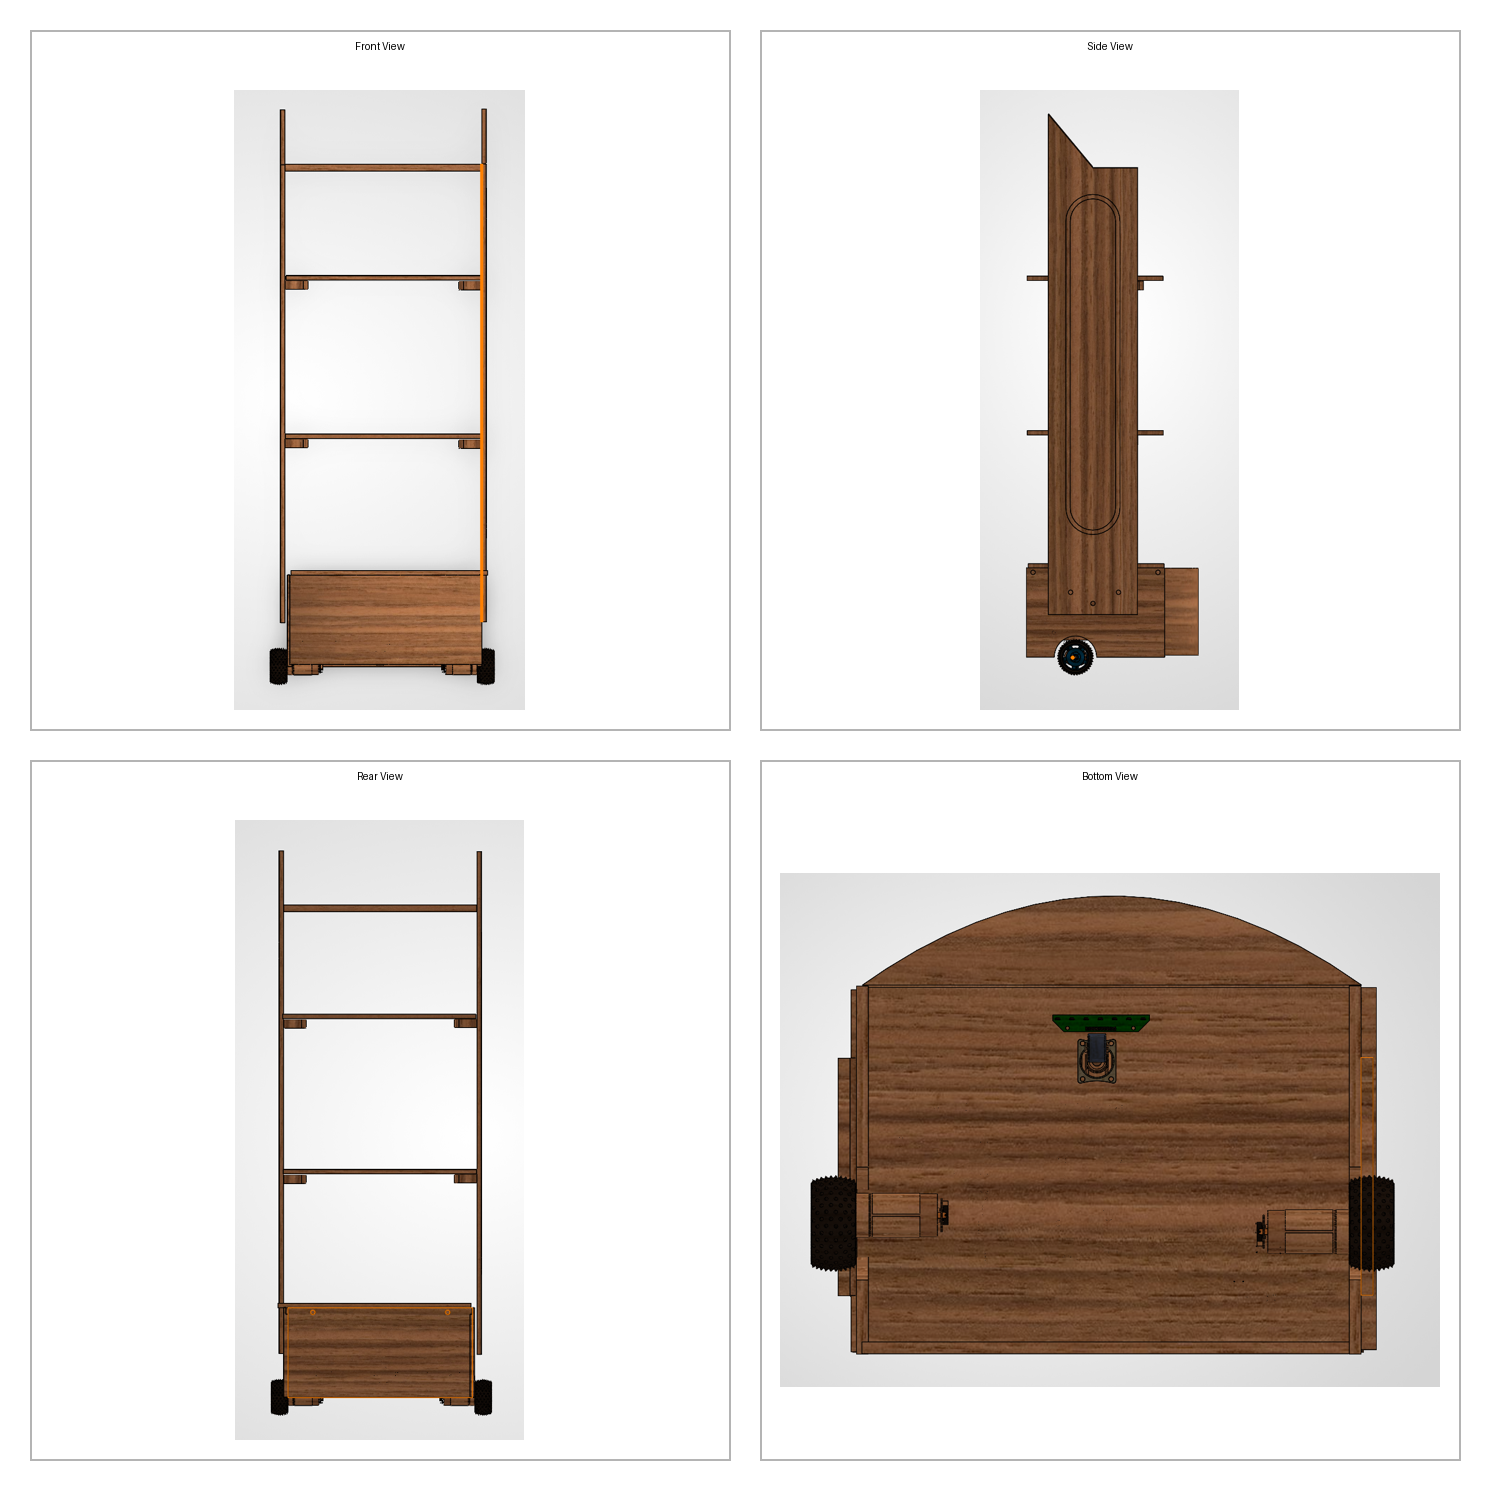
\includegraphics[width=0.6\textwidth]{Robot_Assembly_All_Views.png}
        \caption{Final assembled robot – multiple SOLIDWORKS views}
\end{figure}

%=============================================================
\section{PCB Design}
\label{sec:hardware-design-ref}
%=============================================================

Custom printed circuit boards (PCBs) were designed using Altium
Designer to integrate the electronic subsystems of the Restaurant
Robot. The hardware consists of a main controller board, which
interfaces with all sensors, actuators, and power electronics, and a
shift-register expansion board used for LED control. Designing custom
PCBs improved system integration, reduced wiring complexity, and
enhanced the overall reliability and maintainability of the robot.

\slidefig{altium}
{Altium Designer 3D visualization of the custom printed circuit boards developed for the Restaurant Robot system.}

%-------------------------------------------------------------
\subsection{Main Controller Board}
%-------------------------------------------------------------

The main controller board integrates the ESP32-S3 microcontroller,
power regulation circuitry, motor control interface, and peripheral
connectors into a single compact PCB. Clearly labelled JST connectors
simplify assembly, troubleshooting, and future maintenance.

\begin{itemize}[nosep]
    \item \textbf{M1 / M2} -- Motor outputs for the left and right drive motors.

    \item \textbf{Encoder} -- Motor encoder interface.

    \item \textbf{Array} -- Hall effect sensor array for magnetic tape line following.

    \item \textbf{US1 / US2} -- Ultrasonic sensor interfaces for obstacle detection.

    \item \textbf{Collision} -- Collision (bumper) sensor interface.

    \item \textbf{Display} -- OLED display interface.

    \item \textbf{LED1--LED5} -- LED output connectors.

    \item \textbf{Power} -- Main battery input.
\end{itemize}

%-------------------------------------------------------------
\subsection{Shift-Register Expansion Board}
%-------------------------------------------------------------

A dedicated expansion board incorporates cascaded 74HC595 shift
registers to provide additional digital output channels while reducing
the number of GPIO pins required from the ESP32-S3. The board
interfaces with the LED subsystem through connector groups labelled
\textbf{LC1--LC3}, providing a compact and modular solution for output
expansion.

\slidefig{pcb_expansion_board}
{Shift-register expansion board used for LED output control.}

%-------------------------------------------------------------
\subsection{PCB Connector Allocation}
%-------------------------------------------------------------

Table~\ref{tab:pin-allocation} summarizes the major connectors provided
on the main controller board.

\begin{table}[H]
\centering
\caption{Connector allocation of the Restaurant Robot main controller board.}
\label{tab:pin-allocation}
\renewcommand{\arraystretch}{1.2}
\begin{tabular}{@{}ll@{}}
\toprule
\textbf{Connector} & \textbf{Function} \\
\midrule
M1 / M2 & Left and right motor outputs \\
Encoder & Motor encoder interface \\
Array & Hall effect sensor array \\
US1 / US2 & Ultrasonic sensors \\
Collision & Collision sensor \\
Display & OLED display (I\textsuperscript{2}C) \\
LED1--LED5 & LED output connectors \\
Power & 12 V battery input \\
\bottomrule
\end{tabular}
\end{table}

%-------------------------------------------------------------
\subsection{Fabricated PCB}
%-------------------------------------------------------------

The fabricated PCBs were assembled by soldering the electronic
components onto the manufactured boards. Functional testing confirmed
correct power distribution, peripheral connectivity, and communication
between the ESP32-S3 and the connected sensors and actuators.

\slidefig{pcb}
{Fabricated custom PCBs used in the Restaurant Robot prototype, including the main controller board, power management board, and Hall-effect sensor array PCB.}

%=============================================================
\section{System Integration}
%=============================================================

The final Restaurant Robot prototype was assembled by integrating the
mechanical, electronic, and firmware subsystems into a single
functional platform. The main controller PCB, battery pack, motor
driver, voltage regulators, and other electronic components were
securely mounted within the chassis to ensure structural stability and
ease of maintenance.

Internal wiring was carefully routed to connect the Hall effect sensor
array, ultrasonic sensors, load cell module, motors, OLED display, LED
system, and charging interface to the main controller board. Cable
routing was organized to minimize interference with moving components,
reduce electrical noise, and simplify future maintenance.

Following mechanical assembly, the firmware was uploaded to the
ESP32-S3, and each subsystem was tested individually before performing
full system integration. Successful integration was confirmed through
reliable autonomous navigation, obstacle detection, wireless
communication, load detection, and automatic return-to-charge
operation.

\slidefig{system_internal}
{Internal arrangement of electronic components and wiring inside the robot chassis.}


%=============================================================
\section{Testing}
%=============================================================

A series of functional tests was conducted to verify that the
Restaurant Robot satisfied the design requirements. Each subsystem was
tested individually before evaluating the complete integrated system.
Table~\ref{tab:testing-plan} summarizes the testing procedures.

\begin{table}[H]
\centering
\caption{Summary of system testing procedures.}
\label{tab:testing-plan}
\renewcommand{\arraystretch}{1.3}
\begin{tabular}{@{}p{3.8cm}p{9.2cm}@{}}
\toprule
\textbf{Test} & \textbf{Description} \\
\midrule
Magnetic Line Following &
Verify that the robot accurately follows the magnetic guide tape on the test surface. \\

Obstacle Detection &
Place obstacles along the guide path and verify that the robot stops within the specified detection distance. \\

Weight Detection &
Verify that the load cell correctly detects tray loading and unloading before and after delivery. \\

Wireless Communication &
Verify reliable communication between the tabletop request device, robot, and staff mobile application. \\

Battery Performance &
Measure the operating time on a full charge and verify charging performance. \\

Charging Dock Alignment &
Verify that the robot consistently aligns with and docks at the magnetic pogo-pin charging station. \\

Complete System Test &
Verify the complete delivery sequence, including request reception, autonomous navigation, food delivery, and return to the charging dock. \\
\bottomrule
\end{tabular}
\end{table}

The results obtained from these tests confirmed the correct operation
of the individual subsystems and demonstrated the successful
integration of the complete Restaurant Robot. Representative test
results and performance measurements are presented in the following
subsections.


%=============================================================
\section{Final Product}

\begin{figure}[H]
\centering
\includegraphics[width=0.3\textwidth]{final.png}
\caption{Completed Restaurant Robot prototype.}
\label{fig:comparison}
\end{figure}

%=============================================================

The completed Restaurant Robot prototype integrates the mechanical
structure, embedded electronics, wireless communication system, and
autonomous navigation algorithm into a fully functional food delivery
platform. The final system consists of the autonomous delivery robot,
the tabletop request device, the charging dock, and the staff mobile
application, providing an end-to-end restaurant service solution.


%=============================================================
\section{Power Analysis}
%=============================================================

The Restaurant Robot is powered by a 12~V, 9000~mAh lithium-ion battery,
selected to provide sufficient energy for extended operation during a
typical restaurant service period. The battery supplies power directly
to the drive motors, while onboard voltage regulators provide stable
5~V and 3.3~V outputs for the ESP32-S3, sensors, display, and other
electronic peripherals.

Table~\ref{tab:power-budget} summarizes the power specifications of the
system.

\begin{table}[H]
\centering
\caption{Power budget summary.}
\label{tab:power-budget}
\renewcommand{\arraystretch}{1.2}
\begin{tabular}{@{}p{5cm}p{4cm}p{5cm}@{}}
\toprule
\textbf{Parameter} & \textbf{Value} & \textbf{Description} \\
\midrule
Battery Type & 12 V, 9000 mAh Li-ion & Primary power source \\
Operating Time & 8--10 hours & Continuous operation under normal usage \\
Charging Time & 4--5 hours & Charging via magnetic pogo-pin docking station \\
Motor Supply & 12 V & Direct battery supply \\
Logic Supply & 5 V / 3.3 V & Generated using onboard voltage regulators \\
\bottomrule
\end{tabular}
\end{table}

The drive motors account for the majority of the system's power
consumption, whereas the ESP32-S3, sensors, OLED display, and wireless
communication modules consume comparatively little power. The selected
battery capacity enables the robot to operate continuously throughout a
typical restaurant service session before requiring recharging.
%=============================================================
\section{Cost Analysis}
%=============================================================

\subsection{Prototype Development Cost}

The prototype development cost includes the expenses incurred for
mechanical fabrication, electronic hardware, PCB manufacturing,
battery, motors, sensors, and other essential components required to
build the complete Restaurant Robot prototype.

\begin{table}[H]
\centering
\caption{Prototype development cost breakdown.}
\label{tab:prototype-cost}
\renewcommand{\arraystretch}{1.2}
\begin{tabular}{@{}p{8cm}r@{}}
\toprule
\textbf{Component} & \textbf{Cost (LKR)} \\
\midrule
PCB Manufacturing \& Assembly & 25,000 \\
MCUs (ESP32 + STM32) \& Sensors & 20,000 \\
Passive Components (LCSC) & 20,000 \\
JGB37-555 Motors & 10,000 \\
11.1V 60C 3S LiPo Battery & 10,000 \\
Robot Chassis & 20,000 \\
Magnetic Line & 5,000 \\
LEDs \& 3.5-inch Display & 7,500 \\
\midrule
\textbf{Total Prototype Cost} & \textbf{117,500} \\
\bottomrule
\end{tabular}
\end{table}

%-------------------------------------------------------------
\subsection{Estimated Manufacturing Cost}
%-------------------------------------------------------------

The estimated manufacturing cost for large-scale production is
approximately \textbf{LKR 50,000} per unit. This reduction is achieved
through bulk procurement of electronic components, mass PCB
manufacturing, optimized assembly procedures, and economies of scale,
resulting in a significantly lower production cost compared to the
prototype.

%-------------------------------------------------------------
\subsection{Estimated Selling Price}
%-------------------------------------------------------------

The proposed retail selling price of the Restaurant Robot is
approximately \textbf{LKR 300,000} per unit. This price includes the
manufacturing cost together with assembly, quality assurance,
packaging, transportation, warranty, after-sales support, and the
manufacturer's profit margin.

Compared with commercially available restaurant service robots such as
the BellaBot, which are typically priced between
\textbf{USD 10,000 and USD 20,000}, the proposed system provides a
cost-effective alternative while offering the essential autonomous
food delivery functionality required for restaurants, hotels, and
hospitality environments.

%=============================================================
\section{Business Model and Marketing}
%=============================================================

The Restaurant Robot is intended for commercial deployment in
restaurants seeking to improve service efficiency while reducing staff
workload. The proposed business model combines direct sales and rental
options, enabling restaurants of different sizes to adopt the system
according to their operational requirements.

\slidefig{bis}
{Proposed business model and pricing strategy.}

%-------------------------------------------------------------
\subsection{Pricing Options}
%-------------------------------------------------------------

\begin{table}[H]
\centering
\caption{Proposed pricing options.}
\label{tab:pricing-options}
\renewcommand{\arraystretch}{1.2}
\begin{tabular}{@{}p{7cm}p{5cm}@{}}
\toprule
\textbf{Option} & \textbf{Price} \\
\midrule
One-time purchase (single unit) & LKR 300,000 \\
Monthly rental & LKR 10,000 per month \\
Fleet purchase (5 or more units) & LKR 250,000 per unit \\
\bottomrule
\end{tabular}
\end{table}

%-------------------------------------------------------------
\subsection{Target Customers}
%-------------------------------------------------------------

The proposed system is primarily intended for:

\begin{itemize}[nosep]
    \item Casual dining restaurants.
    \item Hotels and banquet halls.
    \item Cafeterias and food courts.
    \item Hospitality and event venues.
\end{itemize}

%-------------------------------------------------------------
\subsection{Value Proposition}
%-------------------------------------------------------------

The Restaurant Robot offers several advantages over conventional
manual food delivery:

\begin{itemize}[nosep]
    \item Reduces the workload associated with repetitive food
    delivery tasks.

    \item Improves service efficiency by enabling autonomous food
    transportation.

    \item Reduces the likelihood of accidents while carrying food in
    busy restaurant environments.

    \item Provides a modern and interactive dining experience that can
    enhance customer satisfaction.

    \item Allows restaurant staff to focus on higher-value customer
    service activities.
\end{itemize}

%-------------------------------------------------------------
\subsection{Market Readiness}
%-------------------------------------------------------------

The proposed system demonstrates the technical feasibility of an
autonomous restaurant delivery robot. Before commercial deployment,
several additional requirements should be addressed.



\begin{itemize}[nosep]
    \item \textbf{Safety certification:} Compliance with applicable electrical and electronic safety standards.

    \item \textbf{Food-safe materials:} Use of certified food-contact materials for trays and customer-facing components.

    \item \textbf{Floor compatibility:} Validation on a wide range of commercial flooring surfaces.

    \item \textbf{Staff training:} Preparation of operating and maintenance guidelines for restaurant personnel.

    \item \textbf{Regulatory approval:} Compliance with relevant local regulations for commercial equipment.

    \item \textbf{Product support:} Provision of warranty, maintenance, and after-sales services.
\end{itemize}

%=============================================================
\section{Project Challenges and Timeline}
\label{sec:challenges}
%=============================================================

%-------------------------------------------------------------
\subsection{Challenges Encountered}
%-------------------------------------------------------------

Throughout the design and development process, several technical and
practical challenges were encountered. Appropriate engineering
solutions were implemented to overcome these issues and improve the
overall reliability of the system.

\begin{table}[H]
\centering
\caption{Summary of project challenges and implemented solutions.}
\label{tab:project-challenges}
\renewcommand{\arraystretch}{1.3}
\begin{tabular}{@{}p{4.5cm}p{6cm}p{2cm}@{}}
\toprule
\textbf{Challenge} & \textbf{Solution} & \textbf{Status} \\
\midrule
Limited ESP32-S3 GPIO pins &
Implemented a 74HC595 shift-register expansion board &
Resolved \\

5~V ultrasonic sensor output with 3.3~V ESP32 input &
Added a voltage divider to the echo signal &
Resolved \\

Charging dock alignment &
Combined magnetic alignment with pogo-pin charging contacts &
Ongoing \\

Line-following reliability &
Adopted magnetic guide tape with Hall effect sensors &
Resolved \\

Chassis manufacturing cost &
Used wood and commercially available plastic components to reduce fabrication cost &
Partially Resolved \\
\bottomrule
\end{tabular}
\end{table}

%-------------------------------------------------------------
\subsection{Project Timeline}
%-------------------------------------------------------------

\slidefig{timeline}
{Project development timeline from concept to prototype.}

%=============================================================
\section{Future Improvements}
\label{sec:future}
%=============================================================

Although the developed prototype satisfies the primary objectives of
the project, several enhancements can further improve its performance,
flexibility, and commercial viability.

\begin{itemize}[nosep]
    \item \textbf{QR-code ordering:} Allow customers to access menus
    and place orders by scanning a QR code at the table.

    \item \textbf{Customer mobile application:} Develop a dedicated
    mobile application for order tracking and service requests.

    \item \textbf{Voice interaction:} Integrate voice recognition for
    hands-free customer requests.

    \item \textbf{Autonomous mapping:} Replace fixed magnetic guide
    paths with SLAM-based navigation for greater flexibility.

    \item \textbf{Improved charging dock:} Enhance the docking
    mechanism to achieve more reliable autonomous charging.

    \item \textbf{AI-assisted navigation:} Incorporate computer vision
    and intelligent path planning for improved obstacle avoidance and
    dynamic navigation.
\end{itemize}

%=============================================================
\section{Conclusion}
%=============================================================

This project presented the design and development of the
\textbf{Restaurant Robot}, an autonomous food delivery system intended
to improve operational efficiency in restaurants. The complete system
integrates an ESP32-S3-based embedded controller, magnetic tape line
following using Hall effect sensors, ultrasonic obstacle detection, a
load cell-based delivery verification system, wireless communication,
a tabletop request device, and a custom-designed PCB into a single
integrated platform.

The project successfully demonstrated the feasibility of developing a
low-cost autonomous restaurant service robot using locally available
components and fabrication techniques. The modular hardware and
software architecture simplifies maintenance and future system
expansion while providing reliable autonomous navigation and customer
service functionality.

Although further improvements such as SLAM-based navigation, enhanced
autonomous docking, and AI-assisted obstacle avoidance can be
implemented in future versions, the developed prototype successfully
achieved the primary objectives established at the beginning of the
project. The Restaurant Robot therefore provides a practical
foundation for future commercial development of autonomous food
delivery systems suitable for local restaurant environments.

\end{document}
